\documentclass[conference]{IEEEtran}
\IEEEoverridecommandlockouts
% The preceding line is only needed to identify funding in the first footnote. If that is unneeded, please comment it out.
\usepackage{cite}
\usepackage{amsmath,amssymb,amsfonts}
\usepackage{algorithmic}
\usepackage[draft]{graphicx}
\usepackage{textcomp}
\usepackage{xcolor}
\usepackage{subcaption}

% --- IMPORTANT PACKAGES FOR TIKZ/PGFPLOTS ---
\usepackage{tikz}
\usepackage{pgfplots}
\pgfplotsset{compat=1.17} % or another recent version

\def\BibTeX{{\rm B\kern-.05em{\sc i\kern-.025em b}\kern-.08em
    T\kern-.1667em\lower.7ex\hbox{E}\kern-.125emX}}
\begin{document}

\title{Design and Evaluation of a Hybrid Wireless Sensor Network Combining Cluster-Tree and Mesh Routing}

\author{\IEEEauthorblockN{Nicholas Palmer}
  \IEEEauthorblockA{\textit{Dept. of Electrical and Computer Engineering} \\
    \textit{San Diego State University}\\
    San Diego, CA, USA \\
    npalmer2267@sdsu.edu}

}

\maketitle

\begin{abstract}
  Wireless sensor networks (WSNs) are self-organizing networks of sensor nodes deployed to monitor the environment.
  These networks are typically battery-powered with limited processing and storage capabilities, requiring energy-efficient communication protocols and resilience to node and link failures.
  To address these challenges, we propose a hybrid WSN that combines cluster-tree and mesh routing to enhance network performance.
  We also implement router-bridge nodes to improve energy efficiency between cluster heads.
  We evaluate our hybrid WSN using a Python simulation tool and compare it with existing WSNs.
\end{abstract}

\begin{IEEEkeywords}
  Wireless Sensor Network,  AODV, Cluster tree
\end{IEEEkeywords}


\section*{I.\ INTRODUCTION}
Wireless sensor networks (WSNs) are used in a variety of applications, such as environmental monitoring, industrial automation, healthcare, and increasingly, in consumer devices. The necessity for ease of deployment and lower cost hardware have made WSNs popular in recent years, but they also pose significant challenges in terms of self-organization, energy efficiency, and robustness.

\subsection*{Self-Organization}
Self-organization is a crucial advantage of WSNs, allowing deployments in remote or inaccessible locations, making it impractical to pre-configure infrastructure. Self-organization allows nodes to form a network topology and select routing paths dynamically based on the network conditions and the environment. Building an optimal topology presents many challenges given the dynamic nature of the environment, limited computational resources, and energy resources of most low-cost hardware. Most networks use one of two topologies: a hierarchical cluster-tree or a mesh topology.

\begin{itemize}
  \item \textbf{Cluster-Tree}
        \begin{itemize}
          \item Hierarchical network with a single root node and multiple cluster-heads
          \item Cluster-heads are responsible for routing data to and from their cluster
          \item Centralized routing allows for greater energy efficiency as the routing can be optimized for the entire network
        \end{itemize}
  \item \textbf{Mesh}
        \begin{itemize}
          \item Peer-to-peer network with no central nodes or defined hierarchy
          \item Each node is responsible for routing data to and from its neighbors
          \item Decentralized routing allows for greater robustness to node and link failures as the routing can adapt on-demand to changes in the network topology
        \end{itemize}
\end{itemize}




\begin{itemize}
  \item \textbf{Provide context and motivation:}
        \begin{itemize}
          \item Briefly describe wireless sensor networks and why
                \emph{self-organizing} behavior is important (e.g., large
                scale, no fixed infrastructure, battery-powered nodes).
          \item Explain why topology formation and routing are challenging in
                such networks.
        \end{itemize}
  \item \textbf{State the problem:}
        \begin{itemize}
          \item Discuss limitations of using only a cluster-tree topology or
                only mesh routing (e.g., fragility, overhead, latency,
                energy imbalance).
          \item Motivate the need for a hybrid approach.
        \end{itemize}
  \item \textbf{Present the proposed solution (high level):}
        \begin{itemize}
          \item Introduce the idea of a hybrid cluster-tree + mesh network:
                nodes organize into a cluster-tree but can also use mesh
                links for robust routing.
        \end{itemize}
  \item \textbf{Summarize contributions (bullet list):}
        Typical items might include:
        \begin{itemize}
          \item Design of a hybrid cluster-tree + mesh topology formation
                and routing protocol.
          \item Implementation of the protocol in a simulation platform.
          \item Evaluation of average join time, connectivity, packet
                delivery, and energy-related behavior under node and link
                losses.
        \end{itemize}
  \item \textbf{Outline of the paper:}
        \begin{itemize}
          \item Conclude with a short paragraph describing the organization
                of the paper.
        \end{itemize}
\end{itemize}

\vspace{1em}
\section*{II.\ RELATED WORK}

In this section, show awareness of prior work and
position your design with respect to it. Specifically:

\begin{itemize}
  \item \textbf{Summarize relevant literature:}
        \begin{itemize}
          \item Describe existing cluster-tree protocols (e.g., ZigBee-like
                approaches).
          \item Describe mesh routing protocols in sensor/IoT networks.
          \item Mention any known hybrid or hierarchical approaches that
                combine tree and mesh ideas.
        \end{itemize}
  \item \textbf{Highlight limitations of prior work:}
        \begin{itemize}
          \item Explain what existing solutions do not address (e.g.,
                limited robustness to node failures, no analysis of join
                time, no energy-aware design).
        \end{itemize}
  \item \textbf{Position the current work:}
        \begin{itemize}
          \item Clearly state how the proposed hybrid design differs from
                and/or extends prior work and what aspects it focuses on
                (e.g., join time, connectivity under failures, impact of
                energy depletion).
        \end{itemize}
\end{itemize}

\vspace{1em}
\section*{III.\ SYSTEM MODEL AND ASSUMPTIONS}

This section defines the environment in which the protocol operates.
You  should clearly state all assumptions:

\begin{itemize}
  \item \textbf{Network model:}
        \begin{itemize}
          \item Number and types of nodes (e.g., one sink/root, cluster
                heads, regular sensor nodes).
          \item Radio abstraction (single channel, common transmission
                range, interference model at a high level).
          \item Whether nodes are static or mobile (typically static).
        \end{itemize}
  \item \textbf{Traffic model:}
        \begin{itemize}
          \item What traffic is generated (e.g., periodic sensing towards
                the sink, control only, or both).
          \item Which nodes generate data and at what rate.
        \end{itemize}
  \item \textbf{Energy model:}
        \begin{itemize}
          \item Briefly describe the radio states (TX/RX/IDLE/SLEEP) and
                that energy is consumed based on time spent in each state.
          \item State that nodes start with a finite energy budget and shut
                down when energy reaches zero.
        \end{itemize}
  \item \textbf{Additional assumptions and scope:}
        \begin{itemize}
          \item Assumptions on initial energy equality, absence of obstacles,
                simplified propagation or MAC model, etc.
          \item What is deliberately \emph{not} modeled (e.g., no detailed
                interference modeling, no mobility).
        \end{itemize}
\end{itemize}

\vspace{1em}
\section*{IV.\ HYBRID CLUSTER-TREE + MESH NETWORK DESIGN}

This section describes the proposed protocol in detail.

\subsection {Overall Architecture}

\begin{itemize}
  \item Describe the roles of different nodes:
        \begin{itemize}
          \item Sink/root node.
          \item Cluster heads (parents).
          \item Regular/leaf nodes.
          \item Local neighborhood and mesh neighbors
        \end{itemize}
  \item Explain how the cluster-tree and mesh components coexist:
        \begin{itemize}
          \item Cluster-tree provides hierarchical structure and basic
                connectivity.
          \item Discuss  the formation of cluster tree, the role of routers,  cluster overlaps
          \item Mesh  provides improved robustness in the local neighborhood.
        \end{itemize}

\end{itemize}

A  high-level figure illustrating the architecture (tree backbone with some cross-layer mesh links) if given in Figure \ref{fig:highLevel}.

\begin{figure}[t]
  \centering
  \includegraphics[width=\linewidth]{fig1.png}
  \caption{A high-level architecture of the Hybrid Cluster Tree Mesh Network}
  \label{fig:highLevel}
\end{figure}

\subsection{Energy Consumption Model}
Each node is equipped with a CC2420-like radio transceiver. We model the
energy consumption of the radio using four main states: transmit (TX),
receive (RX), idle listening (IDLE), and sleep (SLEEP). Each state $s$
is associated with a constant power draw $P_s$, derived from the
typical CC2420 current consumption and supply voltage.

Let $E_i(t)$ denote the remaining energy of node $i$ at time $t$. Over a
time interval $[t, t+\Delta t]$, the energy is updated according to

\begin{equation}
  E_i(t + \Delta t) = E_i(t) -
  \sum_{s \in \{\mathrm{TX}, \mathrm{RX}, \mathrm{I}, \mathrm{S}\}}
  P_s \, T_{i,s}(t, t+\Delta t).
  \label{eq:energy_update}
\end{equation}

where $T_{i,s}(t,t+\Delta t)$ is the time spent by node $i$ in state
$s$ during $[t, t+\Delta t]$.

Your simulator tracks the radio state ( you have only implemented RX and TX states I believe. Also mention the other radio states of
each node and discuss how your simulator integrates the corresponding energy consumption over
time.

\subsection*{B.\ Network Formation Procedure}

Describe, step by step, how the network forms from an initial empty state:

\begin{itemize}
  \item \textbf{Initial conditions:}
        \begin{itemize}
          \item Describe how the root starts the network and begins  advertising its presence.
        \end{itemize}
  \item \textbf{Discovery and joining:}
        \begin{itemize}
          \item How new nodes detect neighbors or beacons.
          \item How a node chooses a parent or cluster head (e.g., based on
                signal strength, hop count, or node ID).
          \item The message exchange for joining .
        \end{itemize}
  \item \textbf{Cluster formation rules:}
        \begin{itemize}
          \item Conditions for becoming a cluster head versus joining as a
                child.
          \item Any limits on the number of children per cluster head.
        \end{itemize}
  \item \textbf{Timing and re-tries:}
        \begin{itemize}
          \item When and how often nodes attempt to join or re-join if
                the first attempt fails.
        \end{itemize}
\end{itemize}

\subsection*{C.\ Routing Strategy}

This subsection explains how packets are forwarded once the network is
formed:

\begin{itemize}
  \item \textbf{Intra-cluster routing:}
        \begin{itemize}
          \item How children send data to their cluster head and how the
                cluster head forwards data within the cluster (if needed).
        \end{itemize}
  \item \textbf{Inter-cluster/global routing:}
        \begin{itemize}
          \item Default tree-based paths towards the sink (parent-to-parent).
          \item When and how mesh links are used .
        \end{itemize}
  \item \textbf{Route selection:}
        \begin{itemize}
          \item The metric used to choose routes (e.g., hop count, link
                quality, or combined metrics).
          \item What routing information each node stores (parent, cluster
                ID, mesh neighbors, distance to sink, etc.).
        \end{itemize}
\end{itemize}

\subsection*{D.\ Self-Organization and Maintenance}

Describe how the network adapts over time:

\begin{itemize}
  \item \textbf{Handling node failures:}
        \begin{itemize}
          \item How children detect that their parent or cluster head has
                failed (e.g., missed heartbeats or timeouts).
          \item How nodes attempt to re-join the network or select a new
                parent.
        \end{itemize}
  \item \textbf{Handling changing link quality:}
        \begin{itemize}
          \item How link quality is monitored and how bad links lead to
                route changes or parent switches.
        \end{itemize}
  \item \textbf{Mesh adaptation:}
        \begin{itemize}
          \item Rules for creating and removing mesh links between nodes.
          \item Any periodic neighbor discovery or link probing.
          \item The role of routers to provide communication between clusters
        \end{itemize}
  \item \textbf{Energy-related aspects (if applicable):}
        \begin{itemize}
          \item Any mechanisms to reduce energy usage (e.g., sleep cycles,
                rotation of cluster-head roles).
          \item Adaptive Tx Power to reduce energy consumption
          \item Recovery from node failures due to nodes running out of energy -- any proactive algorithmic solution you can offer
        \end{itemize}
\end{itemize}

\vspace{1em}
\section*{V.\ SIMULATION PLATFORM AND EXPERIMENTAL SETUP}

\subsection*{A.\ Simulation Platform}

Describe where and how the protocol is implemented:

\begin{itemize}
  \item Briefly explain the main modules:
        \begin{itemize}
          \item Node and radio abstraction.
          \item Topology and neighbor management.
          \item Protocol logic (formation, routing, maintenance).
          \item Logging and statistics collection.
        \end{itemize}
  \item Note any simplifications:

\end{itemize}

\subsection*{B.\ Scenario Configuration}

This subsection defines the experimental scenarios in detail:

\begin{itemize}
  \item \textbf{Topology:}
        \begin{itemize}
          \item Number of nodes (e.g., 25, 50, 100, 200).
          \item Deployment area size (e.g., $100\,\mathrm{m} \times 100\,\mathrm{m}$).
          \item Node placement (random uniform, grid, etc.).
        \end{itemize}
  \item \textbf{Radio parameters:}
        \begin{itemize}
          \item Communication range or path-loss model. Simplify the discussion here , radio access is based on the distance between nodes.
          \item Assumptions about interference ( we did not have any interference,  what else).
        \end{itemize}
  \item \textbf{Traffic configuration:}
        \begin{itemize}
          \item Packet generation rate (low/medium/high traffic).
          \item Packet size and destinations (root or any destination).
        \end{itemize}
  \item \textbf{Energy configuration:}
        \begin{itemize}
          \item Initial energy per node.
          \item Power levels used in the energy model (TX/RX/IDLE/SLEEP). [You are spending energy only when you receive and Transmit.  Ideally you should have 4 states at least]
        \end{itemize}
  \item \textbf{Failure scenarios (if studied):}
        \begin{itemize}
          \item Patterns and percentages of node failures (random vs targeted).
          \item Link loss or packet loss probabilities, the impact on the network formation and run.
        \end{itemize}
\end{itemize}

\subsection*{C.\ Metrics}

Define clearly what do you  measure and how: Add a plot where it is necessary to show experimental results.

\begin{itemize}
  \item \textbf{Join-related metrics:}
        \begin{itemize}
          \item Per-node join time and average join time.
          \item Join success rate (fraction of nodes that join within a time
                limit).
        \end{itemize}
  \item \textbf{Connectivity metrics:}
        \begin{itemize}
          \item Fraction of nodes with a valid route to the sink.
          \item Average hop count from connected nodes to the sink.
        \end{itemize}
  \item \textbf{Routing performance:}
        \begin{itemize}
          \item Packet delivery ratio (PDR) under various link and node conditions.
          \item End-to-end delay (mean, possibly percentiles) under various link and node conditions.
        \end{itemize}
  \item \textbf{Energy metrics:}
        At the beginning of each experiment, all nodes are initialized with a
        finite energy budget $E_i(0) = E_0$. When the remaining energy of node
        $i$ reaches zero or becomes negative, i.e., $E_i(t) \le 0$, the node is
        permanently disabled. A disabled node turns off its radio and ceases
        all communication and protocol participation. As a result, energy
        depletion induces node losses that may fragment the topology and
        degrade connectivity.

        In addition to per-node energy, the simulator records the cumulative
        time that each node spends in TX, RX, IDLE, and SLEEP. This will enable a
        fine-grained analysis of the energy cost incurred by different network
        roles (e.g., cluster heads, mesh forwarders, routers, and leaf nodes).

        \begin{itemize}
          \item Average remaining energy over time.
          \item Node lifetime (time until individual nodes die).
          \item Network lifetime (time until a threshold fraction of nodes
                is no longer connected).
        \end{itemize}
\end{itemize}
\subsection*{D.\ Experiment Design}

Finally, you should explain how experiments are organized:

\begin{figure}
  \centering
  % Replace with your actual file
  \includegraphics[width=0.9\columnwidth]{fig1.png}
  \caption{Average join time versus network size.}
  \label{fig:jointime}
\end{figure}


\begin{figure}
  \centering
  % Replace with your actual file
  \includegraphics[width=0.9\columnwidth]{fig1.png}
  \caption{Nodes killed versus number of nodes disconnected}
  \label{fig:nodes_killed}
\end{figure}



\begin{itemize}
  \item \textbf{Baseline experiments:}
        \begin{itemize}
          \item Vary network size (e.g., 25--200 nodes) under normal
                conditions to study join time, routing performance, and basic
                scalability.
        \end{itemize}
  \item \textbf{Failure experiments:}
        \begin{itemize}
          \item Introduce node failures (random and/or targeted) and measure
                the effect on connectivity, routing, and join/re-join
                behavior.
          \item {Simulate a scenario where N nodes are killed after the simulation converged to a topology and nodes stay off for some time specified. Nodes are reactivated after being off for some time. Discuss topology changes after the nodes are deactivated and reactivated. }
          \item Introduce packet/link loss and analyze PDR and delay.
        \end{itemize}
  \item \textbf{Energy experiments:}
        \begin{itemize}
          \item Vary initial energy budgets and traffic loads to study the
                trade-off between throughput and network lifetime.
        \end{itemize}

  \item \textbf{Energy-Aware Experiment Design}
        We design several experiments to characterize the impact of energy
        consumption on network connectivity and performance.

        \subsubsection{Network Lifetime vs. Initial Energy}
        In the first experiment set, we investigate how the initial energy
        budget affects the overall network lifetime. The number of nodes, node
        placement, and traffic pattern are kept constant, while the initial
        energy $E_0$ is varied across multiple scenarios (e.g., low, medium,
        and high battery capacity). For each scenario, we record:
        \begin{itemize}
          \item the time of the first node death,
          \item the time at which $10\%$, $50\%$, and $90\%$ of the nodes have
                depleted their energy, and
          \item the time at which the fraction of nodes with a valid route to
                the sink falls below a given connectivity threshold (e.g.,
                $80\%$).
        \end{itemize}
        We refer to the latter as the \emph{network lifetime}, since it
        captures the time interval during which the network remains
        operational from the application point of view.

        \begin{figure}[t]
          \centering
          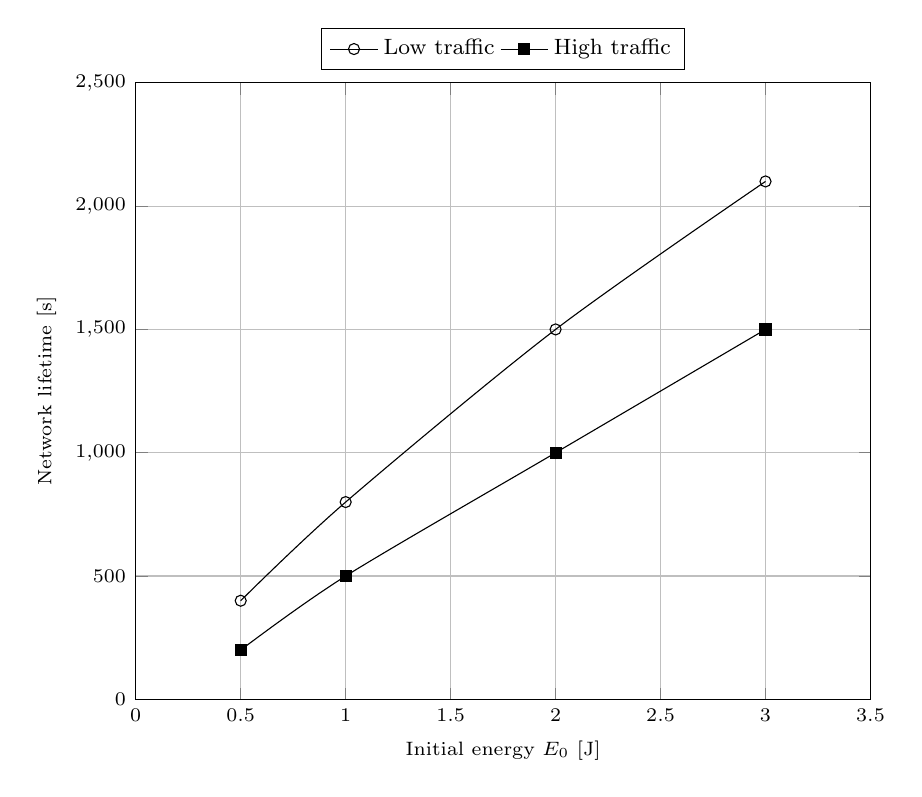
\begin{tikzpicture}
            \begin{axis}[
                width=0.9\columnwidth,
                xlabel={Initial energy $E_0$ [J]},
                ylabel={Network lifetime [s]},
                xmin=0, xmax=3.5,
                ymin=0, ymax=2500,
                grid=both,
                legend style={font=\footnotesize, at={(0.5,1.02)},anchor=south,legend columns=-1},
                tick label style={font=\scriptsize},
                label style={font=\scriptsize}
              ]
              % Low traffic
              \addplot[smooth, mark=o] coordinates {
                  (0.5,400) (1.0,800) (2.0,1500) (3.0,2100)
                };
              \addlegendentry{Low traffic}

              % High traffic
              \addplot[smooth, mark=square*] coordinates {
                  (0.5,200) (1.0,500) (2.0,1000) (3.0,1500)
                };
              \addlegendentry{High traffic}
            \end{axis}
          \end{tikzpicture}
          \caption{Network lifetime as a function of the initial energy budget $E_0$
            per node, for different traffic loads. Network lifetime is defined as the
            time until fewer than $80\%$ of the nodes remain connected to the sink.}
          \label{fig:lifetime_vs_energy}
        \end{figure}


        \begin{figure}[t]
          \centering
          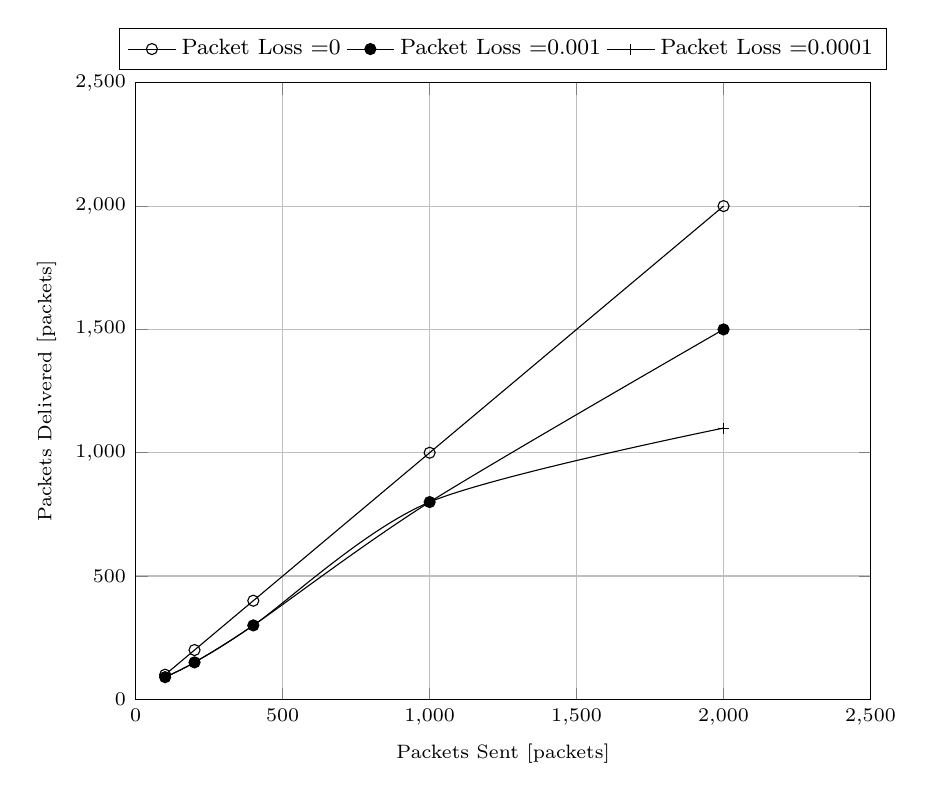
\begin{tikzpicture}
            \begin{axis}[
                width=0.9\columnwidth,
                xlabel={Packets Sent [packets]},
                ylabel={Packets Delivered [packets]},
                xmin=0, xmax=2500,
                ymin=0, ymax=2500,
                grid=both,
                legend style={font=\footnotesize, at={(0.5,1.02)},anchor=south,legend columns=-1},
                tick label style={font=\scriptsize},
                label style={font=\scriptsize}
              ]
              \addplot[smooth, mark=o] coordinates {
                  (100,100) (200,200) (400,400) (1000,1000) (2000,2000)
                };
              \addlegendentry{Packet Loss =0}

              \addplot[smooth, mark=*]
              coordinates {
                  (100,90) (200,150) (400,300) (1000,800) (2000,1500)
                };            \addlegendentry{Packet Loss =0.001}


              \addplot[smooth, mark=+]
              coordinates {
                  (100,90) (200,150) (400,300) (1000,800) (2000,1100)
                };
              \addlegendentry{Packet Loss =0.0001}

            \end{axis}
          \end{tikzpicture}
          \caption{Network lifetime as a function of the initial energy budget $E_0$
            per node, for different traffic loads. Network lifetime is defined as the
            time until fewer than $80\%$ of the nodes remain connected to the sink.}
          \label{fig:packetLossRateIMpact}
        \end{figure}

        \begin{figure}[t]
          \centering
          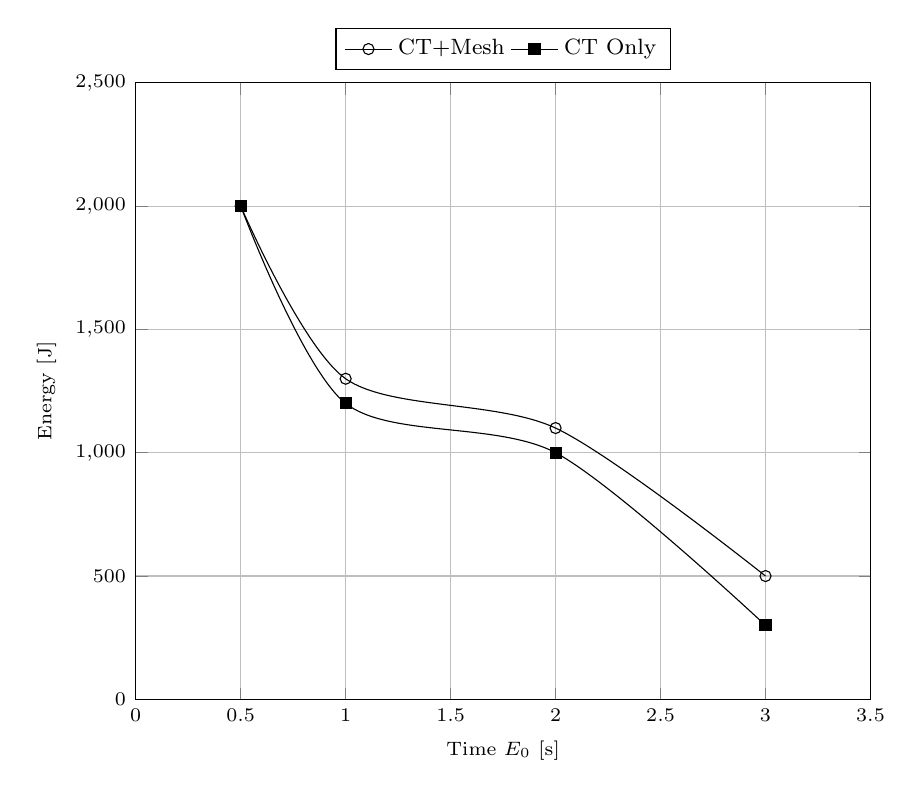
\begin{tikzpicture}
            \begin{axis}[
                width=0.9\columnwidth,
                xlabel={Time $E_0$ [s]},
                ylabel={Energy [J]},
                xmin=0, xmax=3.5,
                ymin=0, ymax=2500,
                grid=both,
                legend style={font=\footnotesize, at={(0.5,1.02)},anchor=south,legend columns=-1},
                tick label style={font=\scriptsize},
                label style={font=\scriptsize}
              ]
              % Low traffic
              \addplot[smooth, mark=o] coordinates {
                  (0.5,2000) (1.0,1300) (2.0,1100) (3.0,500)
                };
              \addlegendentry{CT+Mesh}

              % High traffic
              \addplot[smooth, mark=square*] coordinates {
                  (0.5,2000) (1.0,1200) (2.0,1000) (3.0,300)
                };
              \addlegendentry{CT Only}
            \end{axis}
          \end{tikzpicture}
          \caption{Network lifetime as a function of the initial energy budget $E_0$
            per node, for different traffic loads. Network lifetime is defined as the
            time until fewer than $80\%$ of the nodes remain connected to the sink.}
          \label{fig:energy_comparison}
        \end{figure}



        \begin{figure}[t]
          \centering
          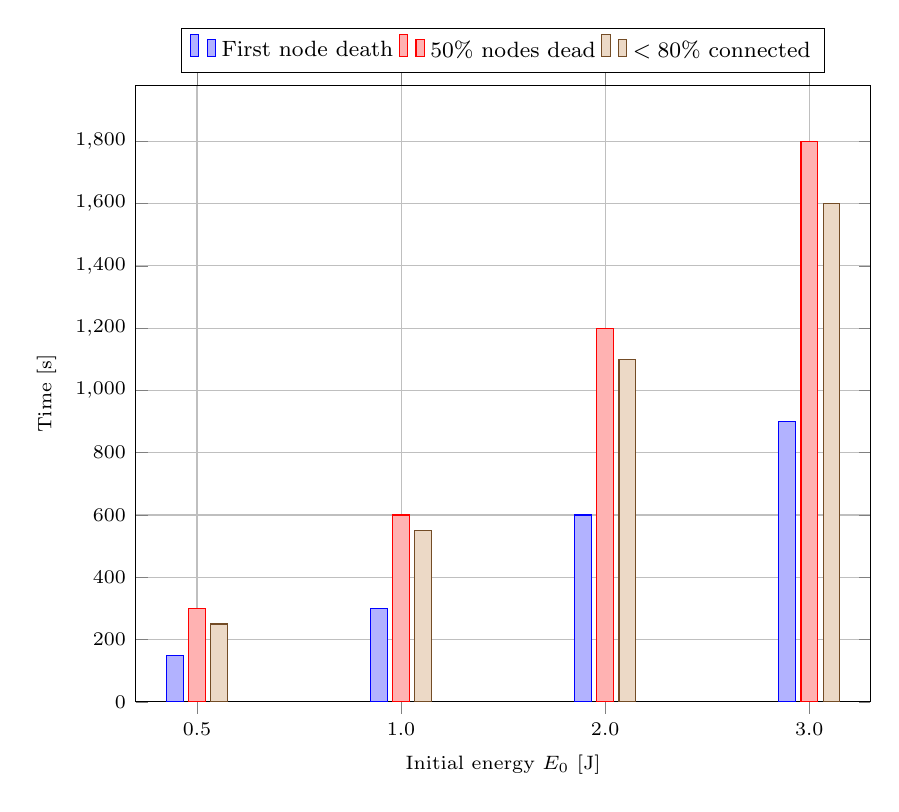
\begin{tikzpicture}
            \begin{axis}[
                width=0.9\columnwidth,
                ybar,
                bar width=6pt,
                xlabel={Initial energy $E_0$ [J]},
                ylabel={Time [s]},
                symbolic x coords={0.5,1.0,2.0,3.0},
                xtick=data,
                ymin=0,
                grid=both,
                legend style={font=\footnotesize, at={(0.5,1.02)},anchor=south,legend columns=3},
                tick label style={font=\scriptsize},
                label style={font=\scriptsize}
              ]
              % First node death
              \addplot coordinates {(0.5,150) (1.0,300) (2.0,600) (3.0,900)};
              \addlegendentry{First node death}

              % 50% nodes dead
              \addplot coordinates {(0.5,300) (1.0,600) (2.0,1200) (3.0,1800)};
              \addlegendentry{50\% nodes dead}

              % Connectivity < 80% (network lifetime)
              \addplot coordinates {(0.5,250) (1.0,550) (2.0,1100) (3.0,1600)};
              \addlegendentry{$<80\%$ connected}
            \end{axis}
          \end{tikzpicture}
          \caption{Impact of the initial energy budget $E_0$ on different lifetime
            metrics: time of first node death, time at which 50\% of the nodes are
            dead, and time at which fewer than 80\% of the nodes remain connected
            to the sink.}
          \label{fig:lifetime_metrics_vs_energy}
        \end{figure}

        \subsubsection{Role-Based Energy Depletion}
        In the second experiment set, we analyze the energy consumption of
        different node roles in the hybrid cluster-tree and mesh topology.
        Cluster heads and mesh forwarders are expected to relay a larger
        fraction of the traffic and to transmit more control packets than leaf
        nodes. To quantify this effect, we log for each node its role, time of
        death (if any), and total time spent in each radio state. We then
        compare:
        \begin{itemize}
          \item the average lifetime of cluster heads and mesh forwarders
                against that of leaf nodes, and
          \item the average energy breakdown (TX/RX/IDLE/SLEEP) per role.
        \end{itemize}
        This experiment highlights whether critical nodes (e.g., cluster heads)
        tend to deplete their batteries prematurely and how their failure
        impacts the remaining topology.

        \subsubsection{Impact of Traffic Load on Energy Consumption}
        In the third experiment set, we study the trade-off between traffic
        load and network lifetime. The topology and initial energy $E_0$ are
        kept fixed, while the application data rate is varied (e.g., low,
        medium, and high packet generation rates per node). For each traffic
        level, we monitor:
        \begin{itemize}
          \item the average remaining energy over time,
          \item the number and fraction of alive nodes,
          \item the number and fraction of nodes with a route to the sink, and
          \item the packet delivery ratio (PDR) computed over sliding time
                windows.
        \end{itemize}
        By comparing these metrics across traffic configurations, we evaluate
        how increased load accelerates energy depletion and reduces the time
        for which the network can sustain a target connectivity or reliability
        level.

        \subsubsection{Energy-Aware vs. Baseline Configuration (Optional)}
        If applicable, we also consider an energy-aware configuration of the
        hybrid protocol, in which the cluster-head role is periodically
        rotated or the maximum number of children per cluster head is limited.
        We compare this configuration against a baseline with fixed cluster
        heads. The comparison focuses on node lifetime distributions, the
        fraction of prematurely dead cluster heads, and the resulting network
        lifetime.

  \item \textbf{Repetitions and statistics:}
        \begin{itemize}
          \item Indicate how many runs are performed per scenario (e.g., 10
                or 20 runs with different random seeds).
          \item Explain how averages and confidence intervals are computed.
        \end{itemize}
\end{itemize}
\subsection{Discussion}

% overall robustness and trade-offs
\subsection{Impact of Energy Consumption on Network Connectivity}
This section presents the impact of energy consumption and
energy-driven node failures on the hybrid cluster-tree and mesh
network.

\subsubsection{Evolution of Alive and Connected Nodes}
Fig.\ref{fig:connectivity_vs_time_traffic} shows the fraction of alive
nodes and the fraction of nodes that maintain a valid route to the
sink as a function of time, for different initial energy budgets
$E_0$. In all cases, the fraction of alive nodes decreases gradually as
nodes deplete their batteries. However, the fraction of connected
nodes typically decreases more abruptly when critical nodes (e.g.,
cluster heads or mesh forwarders) fail. For small $E_0$, the network
rapidly loses connectivity after the first few cluster-head failures.
Larger energy budgets postpone these critical failures and increase
the time interval during which more than $80\%$ of the nodes remain
connected.

\subsubsection{Node Lifetime Distribution and Role Effects}
Fig.~\ref{fig:lifetime_cdf} depicts `` Cluster heads exhibit significantly shorter lifetimes,
confirming that their higher forwarding and control responsibilities
translate into faster energy depletion. As a result, the first network
partitions are typically triggered by the death of cluster heads.
Leaf nodes, in contrast, often retain a substantial amount of energy
when the network as a whole is already disconnected from the sink.
This imbalance suggests that energy-aware role assignment or rotation
mechanisms could substantially extend network lifetime.

\begin{figure}[t]
  \centering
  % Replace with your actual file
  \includegraphics[width=0.9\columnwidth]{fig1.png}
  \caption{Packet delivery ratio (PDR) over
    time.}
  \label{fig:pdr_over_time}
\end{figure}


\subsubsection{Performance Degradation Due to Energy Depletion}
Fig.~\ref{fig:pdr_over_time} shows the packet delivery ratio (PDR) over
time. We observe that PDR remains close to its nominal value while the
majority of nodes are both alive and connected. Once a sufficient
number of cluster heads and relay nodes have died, PDR drops sharply
even though a non-negligible fraction of nodes are still powered.
This indicates that from the application perspective, the effective
end of the network occurs before the physical exhaustion of all
nodes, reinforcing the importance of connectivity-based lifetime
metrics.


\begin{figure}[t]
  \centering
  % Replace with your actual file
  \includegraphics[width=0.9\columnwidth]{fig1.png}
  \caption{Average remaining energy over time for different traffic loads
    (e.g., low, medium, and high packet generation rates per node). Higher
    traffic accelerates energy depletion and reduces the available energy
    budget of the nodes.}
  \label{fig:energy_traffic}
\end{figure}


\begin{figure}[t]
  \centering
  % Replace with your actual file
  \includegraphics[width=0.9\columnwidth]{fig1.png}
  \caption{Fraction of nodes that remain connected to the sink over time
    for different traffic loads. Under high traffic, connectivity drops
    significantly earlier, reducing the effective network lifetime.}
  \label{fig:connectivity_vs_time_traffic}
\end{figure}


\begin{figure}[t]
  \centering
  % Replace with your actual file
  \includegraphics[width=0.9\columnwidth]{fig1.png}
  \caption{The cumulative distribution
    function (CDF) of node lifetimes, separately for cluster heads and
    leaf nodes.}
  \label{fig:lifetime_cdf}
\end{figure}

\subsubsection{Impact of Traffic Load on Lifetime}
Fig.~\ref{fig:energy_traffic} compares the average remaining energy and
connectivity over time for different traffic loads. Higher packet
generation rates lead to a faster reduction in the average remaining
energy and a correspondingly earlier loss of connectivity. For high
traffic, the network lifetime (time until fewer than $80\%$ of nodes
remain connected) can be reduced by more than half compared to the
low-traffic scenario. This highlights a fundamental trade-off between
throughput and lifetime in the proposed hybrid architecture.

\subsubsection{Comparison with Energy-Aware Configuration (Optional)}
If an energy-aware configuration is enabled, in which cluster-head
roles are periodically rotated or constrained by a maximum number of
children, the lifetime results improve. In our simulations, the
energy-aware configuration shifts the node lifetime CDF for cluster
heads closer to that of leaf nodes and delays the onset of major
connectivity losses. Consequently, the time at which PDR drops below
the target threshold increases, demonstrating that simple
energy-balancing mechanisms can significantly enhance the robustness
of the hybrid cluster-tree and mesh network.

\section{Conclusion and Future Work}
% summary + future work

\bibliographystyle{IEEEtran}
\nocite{*}
\bibliography{references}

\end{document}
